\makeheading{Week 2}{\daterange{2021-09-13}{2021-09-17}}%chktex 8
\section{Module 1: Measures of Disease Frequency}
\subsection{Incidence and Prevalence Rates}
\subsubsection*{How do we measure and evaluate patterns of disease within a population?}
\begin{figure}[H]
    \centering
    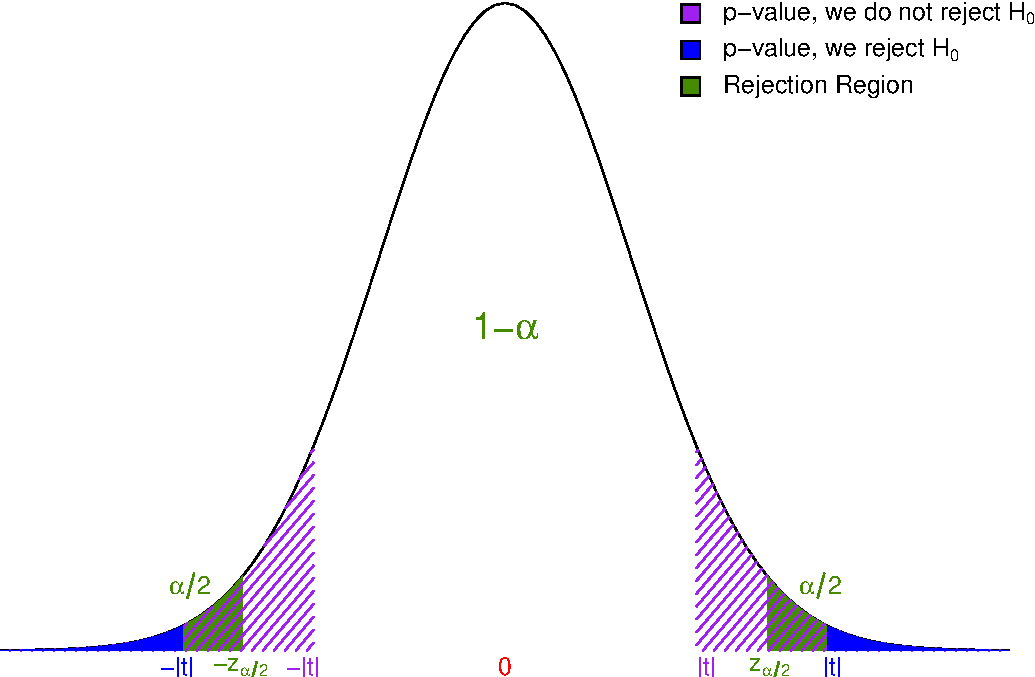
\includegraphics[width=0.75\textwidth]{1.1/1.pdf}
\end{figure}
\subsubsection*{Primer on HIV/AIDS}
\begin{itemize}
    \item HIV (human immunodeficiency virus) is a virus that attack’s the body’s immune
          system.
    \item HIV is spread through sexual contact, sharing needles, and mother-to-child
          transmission during pregnancy, childbirth, or breastfeeding.
    \item Infection with HIV can lead to AIDS (acquired immunodeficiency syndrome).
    \item Individuals with AIDS are at increased risk of infection and infection-related
          cancers.
    \item Currently, no cure exists, but antiretroviral therapy can slow the progression of the
          disease.
\end{itemize}
\subsubsection*{1.1 Incidence and Prevalence Rates}
\begin{Regular}
    \textcolor{Blue}{Goal}: How do we measure and evaluate patterns of disease within a population?
\end{Regular}
\begin{itemize}
    \item \textcolor{Blue}{Prevalence}: The proportion of the population currently affected by a disease.
    \item \textcolor{Blue}{Incidence}: The rate at which new cases of a disease develop in a population.
\end{itemize}
\subsubsection*{Number of people living with HIV/AIDS 1990--2017}
\begin{figure}[H]
    \centering
    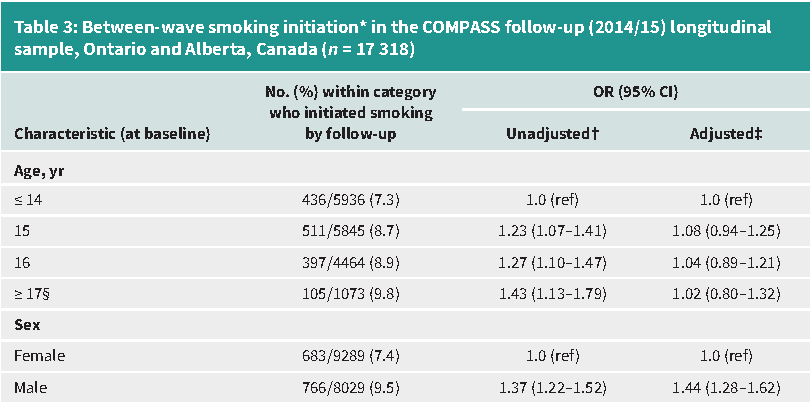
\includegraphics[width=0.75\textwidth]{1.1/2.pdf}
\end{figure}
\subsubsection*{Prevalence}
\textcolor{Blue}{Prevalence}: The proportion of the population currently affected by a disease.
\begin{Regular}
    \[ \begin{tabular}{>{\bfseries}c}
            Point Prevalence \\
            per 1000
        \end{tabular}=\frac{\begin{tabular}{>{\bfseries}c}
                Number of cases (new and pre-existing) in the \\
                population at a fixed point in time
            \end{tabular}}{\begin{tabular}{>{\bfseries}c}
                Number of individuals in the \\
                population at a fixed point in time
            \end{tabular}}\times 1000.  \]
\end{Regular}
\begin{Regular}
    \[ \begin{tabular}{>{\bfseries}c}
            Period Prevalence \\
            per 1000
        \end{tabular}=\frac{\begin{tabular}{>{\bfseries}c}
                Number of cases (new and pre-existing) in the \\
                population over a given time period
            \end{tabular}}{\begin{tabular}{>{\bfseries}c}
                Number of individuals in the \\
                population over a given time period
            \end{tabular}}\times 1000.  \]
\end{Regular}
\subsubsection*{Prevalence of HIV/AIDS 1990--2017}
\begin{figure}[H]
    \centering
    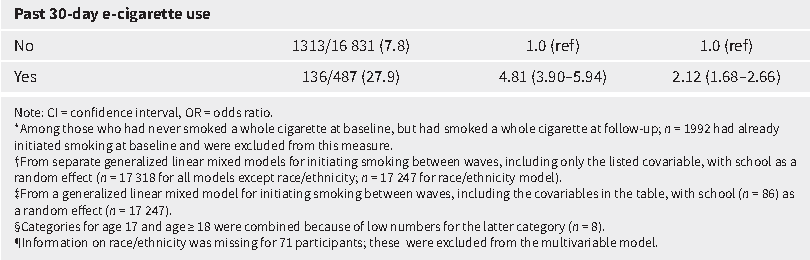
\includegraphics[width=0.75\textwidth]{1.1/3.pdf}
\end{figure}
\subsubsection*{Annual new cases of HIV infection, 1990--2017}
\begin{figure}[H]
    \centering
    \includegraphics[width=0.75\textwidth]{1.1/4.pdf}
\end{figure}
\subsubsection*{Cumulative Incidence}
\textcolor{Blue}{Incidence}: The rate at which \textbf{new cases} of a disease develop in a \textbf{population} over a
specific \textbf{time} period.
\begin{Regular}
    \[ \begin{tabular}{>{\bfseries}c}
            Cumulative Incidence \\
            per 1000
        \end{tabular}=\frac{\begin{tabular}{>{\bfseries}c}
                Number of new cases in the \\
                population over the time period of interest
            \end{tabular}}{\begin{tabular}{>{\bfseries}c}
                Number of individuals at risk in the \\
                population at the start of the time period of interest
            \end{tabular}}\times 1000.  \]
\end{Regular}
\begin{itemize}
    \item Assumes all subjects remain in the population and at risk for the entire time period.
    \item Easily violated: Births, deaths, immigration, emigration, case diagnosis.
    \item Consider two ways to refine the denominator calculation.
          \begin{enumerate}[1.]
              \item Use a mid-interval population estimate.
              \item Calculate the total person-time at risk in the population.
          \end{enumerate}
\end{itemize}
\subsubsection*{Incidence Density or Incidence Rate}
\begin{Regular}
    \[ \begin{tabular}{>{\bfseries}c}
            Incidence Density \\
            per 1000
        \end{tabular}=\frac{\begin{tabular}{>{\bfseries}c}
                Number of new cases in the \\
                population over the time period of interest
            \end{tabular}}{\begin{tabular}{>{\bfseries}c}
                Mid-interval estimate of the population
            \end{tabular}}\times 1000.  \]
\end{Regular}
\begin{Example}
    \begin{itemize}
        \item 3,218 new cases of HIV in Canada, 2016.
        \item 36,264,604 July 1, 2016 Canadian population estimate.
              \[ \begin{tabular}{>{\bfseries}c}
                      Incidence Density \\
                      per 100,000
                  \end{tabular}=\frac{3,218}{36,264,604}\times 100,000=8.873666. \]
        \item \emph{The incidence of HIV infection in Canada in the year 2016 was 8.87 cases per
                  100,000 persons}.
    \end{itemize}
\end{Example}
\subsubsection*{Incidence of HIV per 1,000 uninfected adults, 2000--2017}
\begin{figure}[H]
    \centering
    \includegraphics[width=0.75\textwidth]{1.1/5.pdf}
\end{figure}
\subsubsection*{Person-time at risk}
\begin{itemize}
    \item To account for varying time periods of risk we consider an alternative denominator
          for our incidence calculation.
    \item Person-time at risk is the duration of time an individual is at risk for developing
          a disease.
    \item Assuming they are initially disease free, it is the length of time from baseline until
          the first of:
          \begin{enumerate}[1.]
              \item They develop the disease of interest and become a case.
              \item They cease to be at risk of becoming a case due to either death from unrelated
                    causes or they leave the population.
              \item The end of the time period of interest is reached.
          \end{enumerate}
    \item Total person-time at risk is the sum of the individual contributions over the
          population.
\end{itemize}
\subsubsection*{Incidence Density or Incidence Rate}
\begin{Regular}
    \[ \begin{tabular}{>{\bfseries}c}
            Incidence Density \\
            per 1000
        \end{tabular}=\frac{\begin{tabular}{>{\bfseries}c}
                Number of new cases in the \\
                population over the time period of interest
            \end{tabular}}{\begin{tabular}{>{\bfseries}c}
                Mid-Total person-time at risk in the \\
                population over the time period of interest
            \end{tabular}}\times 1000.  \]
\end{Regular}
\begin{itemize}
    \item Incidence density estimate is more precise than cumulative incidence, but may be
          harder to get information needed, so this measure is often used for small
          populations.
    \item Expressed as per $10^x$ person-years (-month, -day).
\end{itemize}
\subsubsection*{Relationship Between Incidence and Prevalence}
\begin{figure}[H]
    \centering
    \includegraphics[width=0.25\textwidth]{1.1/6.jpg}
\end{figure}
\subsubsection*{Relationship Between Incidence and Prevalence}
\begin{itemize}
    \item \textbf{Incidence}: the rate new cases are diagnosed in a population.
    \item \textbf{Prevalence}: the proportion of the population currently affected by the disease.
\end{itemize}
\begin{Regular}
    \[ \textbf{Prevalence}\approx \textbf{Incidence}\times \textbf{Disease Duration} \]
\end{Regular}
\begin{itemize}
    \item Relationship is approximate but generally holds well if prevalence is low ($<10\,$\%)
          and duration is fairly constant (or an average can be taken).
    \item Note: units must be consistent in order to perform the multiplication operation.
\end{itemize}
\subsubsection*{Prevalence, new cases, and mortality for HIV/AIDS}
\begin{figure}[H]
    \centering
    \includegraphics[width=0.75\textwidth]{1.1/7.pdf}
\end{figure}
\subsubsection*{Exercise: Incidence and Prevalence Calculations}
Total population size of 100. Histories of 12 subjects with disease are below. Subjects
13--100 do not have the disease during the year of study. ($ \triangle $ Diagnosis; $ \times $ Death)
\begin{table}[H]
    \centering
    \begin{tabular}{ccc}
        \toprule
        \textbf{Subject} & \textbf{Diagnosis} $ \triangle $ & \textbf{Death} $ \times $ \\
        \midrule
        1                & $<$ January 1                                                \\
        2                & $<$ January 1                    & April 30                  \\
        3                & $<$ January 1                                                \\
        4                & $<$ January 1                                                \\
        5                & $<$ January 1                    & June 30                   \\
        6                & March 1                          & October 31                \\
        7                & May 1                                                        \\
        8                & May 1                                                        \\
        9                & July 1                                                       \\
        10               & July 1                           & October 31                \\
        11               & NA                               & May 1                     \\
        12               & NA                               & September 1               \\
        13--100          & NA                                                           \\
        \bottomrule
    \end{tabular}
\end{table}
\begin{figure}[H]
    \centering
    \includegraphics[width=0.75\textwidth]{1.1/8.pdf}
\end{figure}
\begin{itemize}
    \item Point Prevalence on July 1.
    \item Period Prevalence (Jan 1 to Dec 31)
    \item Cumulative Incidence (Jan 1 to Dec 31).
    \item Incidence Density (Jan 1 to Dec 31).
\end{itemize}
\begin{align*}
    \begin{tabular}{c}
        Point Prevalence \\
        on July 1
    \end{tabular}
     & =\frac{\text{\# cases in the pop on July 1}}{\text{\# indv in the pop on July 1}}\times 1000=\frac{8}{97}\times 1000=\text{$82.47$ per 1000 persons}.                     \\\\
    \begin{tabular}{c}
        Period Prevalence \\
        (Jan 1-Dec 31)
    \end{tabular}
     & =\frac{\text{\# cases during Jan 1-Dec 31}}{\text{\# indv in the pop Jan 1-Dec 31}}\times 1000=\frac{10}{100}\times 1000=\text{$100$ per 1000 persons}.                   \\\\
    \begin{tabular}{c}
        Cumulative Incidence \\
        (Jan 1-Dec 31)
    \end{tabular}
     & =\frac{\text{\# new cases during Jan 1-Dec 31}}{\text{\# indv at risk on Jan 1}}\times 1000=\frac{5}{95}\times 1000=\text{$52.63$ per 1000 persons}.                      \\\\
    \begin{tabular}{c}
        Incidence Density \\
        (Jan 1-Dec 31)
    \end{tabular}
     & =\frac{\text{\# new cases during Jan 1-Dec 31}}{\text{July 1 population size}}\times 1000=\frac{5}{97}\times 1000=\text{$51.55$ per 1000 persons}.                        \\\\
    \begin{tabular}{c}
        Incidence Density \\
        (Jan 1-Dec 31)
    \end{tabular}
     & =\frac{\text{\# new cases during Jan 1-Dec 31}}{\text{\small Total person-years at risk Jan 1-Dec 31}}\times 1000=\frac{5}{90.83}\times 1000=\text{$55.05$ per 1000 p-y}. \\
\end{align*}
\subsection{Standardization of Rates: Indirect Methods}